\documentclass[article,oneside]{memoir}

\usepackage{graphicx} % Add graphics capabilities
\usepackage{booktabs} % ``Proper'' table layout
\usepackage{amsmath}  % Better maths support
%\usepackage[colorlinks=false,linkcolor=red]{hyperref} % Hyperlink capabilities
\usepackage{url}

\usepackage{memhfixc} % This package is required to resolve incompatibilities
                      % with the memoir class & the hyperref package
                      
\setlength{\oddsidemargin}{ 20pt}
\setlength{\textwidth}{440pt}
\setlength{\topmargin}{ 0pt}
\setlength{\headheight}{00pt}
\setlength{\headsep}{40pt}
\setlength{\textheight}{620pt}

\title {ENEE631 Project 1 \\ Wavelet-Based Image Compression}
\author{Naotoshi Seo, sonots@umd.edu}
\date{April 11, 2007}


\begin{document}

\maketitle


\chapter{Introduction}

Wavelet-based image coding has gone through significant advancement since the DCT-based codec became the first JPEG standard. In this project, we explore the wavelet-based image coding and examine major factors the affect the coding performance. The Embedded Zero-Tree Wavelet (EZW) codec for image compression is implemented. In addition, Block-based EZW coding is implemented and comparison between different block sizes are performed, furthermore, the Block-based EZW coding is compared with the JPEG-like code which was implemented in assignment 3. SPIHT based compression is also experimented. 

\chapter{Literature Survey}

\section{EZW}
The embedded zerotree wavelet (EZW) encode is based on progressive encoding to compress an image into a bit stream with increasing accuracy. This means that when more bits are added to the stream, the decoded image will contain more detail. Coding an image with EZW scheme, an encoder can terminate the encoding at any point thereby allowing a target rate or target distortion metric to be met exactly. Also, give a bit stream, the decoder can cease decoding at any point in the bit stream and still produce exactly the same image that would have been encoded at the bit rate corresponding to the truncated bit stream. 

The EZW algorithm is based on four key concepts: 1) a discrete wavelet transform or hierarchical subband decomposition, 2) prediction of the absence of significant information across scales by exploiting the self-similarity inherent in images, 3) entropy-coded successive approximation quantization, and 4) universal lossless data compression which is achieved via adaptive arithmetic coding \cite{Shapiro}. 


\section{The Wavelet Transform}

Wavelet based techniques for image compression have been increasingly used for image compression. 
The main contribution of wavelet theory is that it provides an elegant framework in which both "anomalies," or signal behavior that is more localized in the time or space domain and tends to be wide band in the frequency domain, and "trends," or signal behavior that is more localized in frequency but persists over a large number of lags in the time domain. 
Wavelets provide a signal representation in which some of the coefficients represent long data lags corresponding to a narrow band, low frequency range, and some of the coefficients represent short data lags corresponding to a wide band, high frequency range. Using the concept of \textit{scale}, data representing a continuous tradeoff between time (or space in the case of images) and frequency is available. 

A comparative study of DCT and wavelet based image coding can be found in \cite{Xiong}. 

\section{SPIHT}

The Set Partitioning in Hierarchical Trees (SPIHT) algorithm is  an extension of the EZW scheme, proposed by A. Said and W. Pearlman in \cite{Said}. SPIHT improves the basic zerotree coding algorithm of EZW by using slightly different tree structures and allowing the zerotree symbols to be generated in more cases (i.e., for combinations of parallel zerotrees). SPIHT achieves more efficient significance map coding because of the set partitioning algorithm (sophisticated method of stepping through and partitioning the sets of trees and coefficients shared by encoder and decoder).

\section{EBCOT}

The Embedded Block Coding with Optimized Truncation (EBCOT) is a scheme which JPEG2000 uses, introduced by David Taubman \cite{Taubman}. The EBCOT algorithm is related to much earlier work such as EZW, SPIHT. Like each of these, the EBCOT algorithm uses a Wavelet transform to generate the subband samples which to be quantized and coded. Like each of these, the EBCOT also generates scalable  compressed bit-streams; however, whereas its predecessors typically exhibited one (SNR) or at most two (SNR and resolution) dimensions of scalability, the EBCOT algorithm produces bit-streams which are SNR and resolution scalable and which also have a random access attribute whereby independent portions of the bit-stream correspond to different spatial regions of the image. 

A key advantage of scalable compression is that the target bit-rate or reconstruction resolution need not be known at the time of compression. Rather than focusing on generating a single scalable bit-stream to represent the entire image, EBCOT partitions each subband into relatively small blocks of samples and generates a separate highly scalable bit-stream to represent each so-called code-block \cite{Taubman}. 

\chapter{Experiments and Results}

\section{EZW}

EZW-based Image Compression was implemented. 
The details of this scheme is availabe on Shapiro's paper \cite{Shapiro}. 
Huffman encoding was used for entropy encoding. 
Comparison between a quadrature mirror filter (QMF)-wavelet and a haar-wavelet was performed. 
As the result, a QMF-wavlet was used. 

 \begin{center}
  \begin{figure}[ht]
  \begin{tabular}{@{} ccc @{}}

  \begin{minipage}{0.33\hsize}
   \begin{center}
   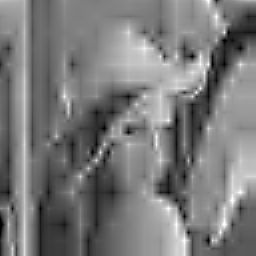
\includegraphics[width=5cm]{../images/LenaEZW04of10.png}\\
   (a)
   \end{center}
  \end{minipage}    &
  \begin{minipage}{0.33\hsize}
   \begin{center}
   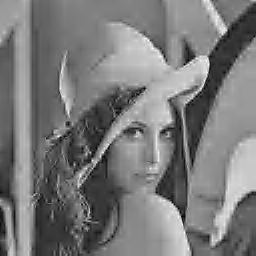
\includegraphics[width=5cm]{../images/LenaEZW06of10.png}\\
   (b)
   \end{center}
  \end{minipage}    &
  \begin{minipage}{0.33\hsize}
   \begin{center}
   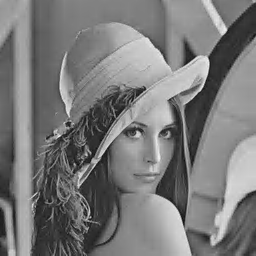
\includegraphics[width=5cm]{../images/LenaEZW08of10.png}\\
   (c)
   \end{center}
  \end{minipage}    \\

  \end{tabular}
 \caption{(a) Decoded image at fourth pass, bpp = 0.0387, PSNR = 21.2866 dB . 
(b) Decoded image at sixth pass, bpp = 0.3179, PSNR = 26.9341 dB . 
(c) Decoded image  at eighth pass, bpp = 1.3424, PSNR = 34.6630 dB . 
 } 
 \label{fig:gabor}
 \end{figure} 
\end{center}

\newpage

\subsection{Comparison between QMF-wavelet and haar-wavelt}

EZW compression using a haar-wavelet and a quadrature mirror filter (QMF)-wavelet were compared. 
As shown in the next figure, a QMF-wavelet is completely better than a haar-wavele which achieved only pretty low (bad) PSNR. 

\begin{center}
\includegraphics[width=14cm]{../src/LenaEZWPlotQMFvsHaar.png}\\
\end{center}


\section{Block-EZW}

Block based EZW coding was also implemented. As a way of implementation, a delimiter symbol was inserted between each block's symbol table generated at the dominant and the subordinate pass, and these symbol tables were connected and encoded at burst using huffman encoding. 
Below pictures show the compressed image at the 1st, 2nd, 3rd pass with block size M = 8. 


 \begin{center}
  \begin{figure}[ht]
  \begin{tabular}{@{} ccc @{}}

  \begin{minipage}{0.33\hsize}
   \begin{center}
   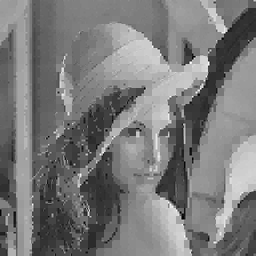
\includegraphics[width=5cm]{../images/LenaBlockEZW01of08M08.png}\\
   (a)
   \end{center}
  \end{minipage}    &
  \begin{minipage}{0.33\hsize}
   \begin{center}
   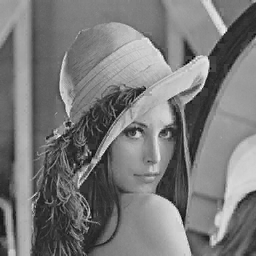
\includegraphics[width=5cm]{../images/LenaBlockEZW03of08M08.png}\\
   (b)
   \end{center}
  \end{minipage}    &
  \begin{minipage}{0.33\hsize}
   \begin{center}
   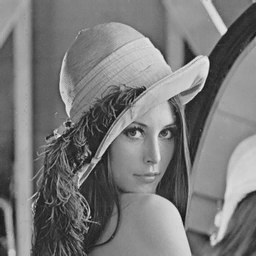
\includegraphics[width=5cm]{../images/LenaBlockEZW05of08M08.png}\\
   (c)
   \end{center}
  \end{minipage}    \\

  \end{tabular}
 \caption
 {
 Block-EZW with block size 32. 
 (a) Decoded image at 1st pass, bpp = 0.0658, PSNR = 21.0563 dB . 
(b) Decoded image at 3rd pass, bpp = 0.4858, PSNR = 27.1965 dB . 
(c) Decoded image  at 5th pass, bpp = 1.7988, PSNR = 34.3224 dB . 
 } 
 \label{fig:gabor}
 \end{figure} 
\end{center}

 \begin{center}
  \begin{figure}[ht]
  \begin{tabular}{@{} ccc @{}}

  \begin{minipage}{0.33\hsize}
   \begin{center}
   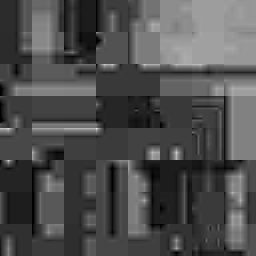
\includegraphics[width=5cm]{../images/circuitBlockEZW01of06M32.png}\\
   (a)
   \end{center}
  \end{minipage}    &
  \begin{minipage}{0.33\hsize}
   \begin{center}
   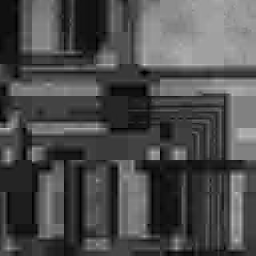
\includegraphics[width=5cm]{../images/circuitBlockEZW02of06M32.png}\\
   (b)
   \end{center}
  \end{minipage}    &
  \begin{minipage}{0.33\hsize}
   \begin{center}
   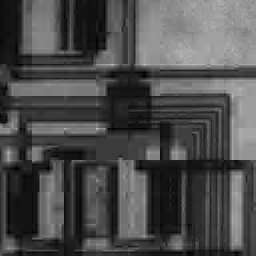
\includegraphics[width=5cm]{../images/circuitBlockEZW03of06M32.png}\\
   (c)
   \end{center}
  \end{minipage}    \\

  \end{tabular}
 \caption
 {
 Block-EZW with block size 32. 
 (a) Decoded image at 1st pass, bpp = 0.7136, PSNR = 24.1599 dB . 
(b) Decoded image at 2nd pass, bpp = 1.9872, PSNR = 28.6582 dB . 
(c) Decoded image  at 3rd pass, bpp = 3.5583, PSNR = 33.6806 dB . 
 } 
 \label{fig:gabor}
 \end{figure} 
\end{center}

\newpage

\subsection{Comparison of different block sizes}

Below figure shows us that larger block size achieved better (less) bits per pixel for the same PSNR. 
This is because EZW encoding is more efficient for larger block (one zerotree symbol represents many coefficients). Notice: smaller block size version also requires more computation for one pass, but requires fewer number of passes to achieve the same PSNR, totally computation time could become almost same. 
In conclusion, the non-Block based default EZW encoding works better. 

\begin{center}
\includegraphics[width=14cm]{../src/LenaEZWPlotBlockSizes.png}\\
Comparison between block size 8, 16, 32 and non-block version of EZW. 
\end{center}

\subsection{Comparison between Block-EZW and JPEG-like codec}

The block size of the JPEG-like codec assignment 3 is fixed 8, thus we compare them with the block size 8. 
Block-EZW requires pretty much bpp even in the first pass when the block size is 8. 
Because of this reason, Block-EZW with block size 8 was pretty worse than the JPEG-like codec. 

The JPEG-like codec uses DCT transform. 
In the case of DCT, the block size compensates tradeoffs between the spatial resolution and the frequency resolution. 
However, in the case of Block-EZW, it resulted in only disadvantages. 
This is because EZW uses wavelet transform which originally provides an elegant framework in which both anomalies and trends. \cite{Shapiro}. 

\section{SPIHT}

SPIHT Matlab code \cite{SPIHT} library was used. 
SPIHT did not have fine adjustments of target bpp, the least bpp was 0.4377 and the most bpp was 7.5886. Even if bpp = 0.01 is specified, the resulted bpp was 0.4377, and even if bpp = 15 is specified, the resulted bpp was 7.5886. 


 \begin{center}
  \begin{figure}[ht]
  \begin{tabular}{@{} ccc @{}}

  \begin{minipage}{0.33\hsize}
   \begin{center}
   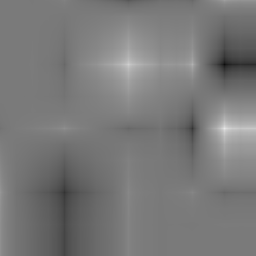
\includegraphics[width=5cm]{../images/LenaSPIHT01.png}\\
   (a)
   \end{center}
  \end{minipage}    &
  \begin{minipage}{0.33\hsize}
   \begin{center}
   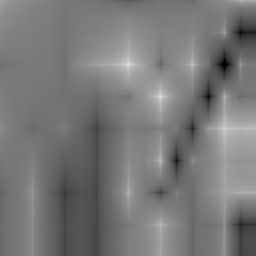
\includegraphics[width=5cm]{../images/LenaSPIHT02.png}\\
   (b)
   \end{center}
  \end{minipage}    &
  \begin{minipage}{0.33\hsize}
   \begin{center}
   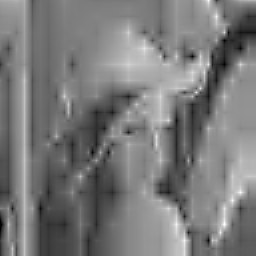
\includegraphics[width=5cm]{../images/LenaSPIHT03.png}\\
   (c)
   \end{center}
  \end{minipage}    \\
  
    \begin{minipage}{0.33\hsize}
   \begin{center}
   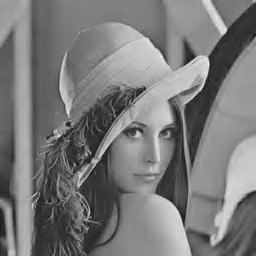
\includegraphics[width=5cm]{../images/LenaSPIHT04.png}\\
   (d)
   \end{center}
  \end{minipage}    &
  \begin{minipage}{0.33\hsize}
   \begin{center}
   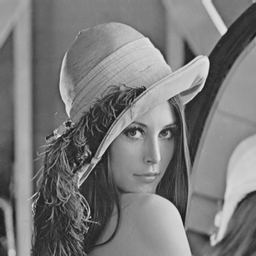
\includegraphics[width=5cm]{../images/LenaSPIHT05.png}\\
   (e)
   \end{center}
  \end{minipage}    &  \\

  \end{tabular}
 \caption
 {
SPIHT. 
 (a) Decoded image at 1st pass, bpp = 0.4377, PSNR = 15.3562 dB . 
(b) Decoded image at 2nd pass, bpp = 0.8754, PSNR = 16.4917 dB . 
(c) Decoded image  at 3rd pass, bpp = 1.7541, PSNR = 20.7105 dB . 
(d) Decoded image  at 4th pass, bpp = 3.7656, PSNR = 33.3704 dB . 
(e) Decoded image  at 5th pass, bpp = 7.5886, PSNR = 45.3426 dB . 
 } 
 \label{fig:gabor}
 \end{figure} 
\end{center}

\newpage



\chapter{Lists of codes}


\section{EZW}

\begin{itemize}
\item ezw.m - EZW encoding
\item ezw\_dominantpass.m - performs dominant pass of ezw encoding, used by ezw.m
\item ezw\_subordiantepass.m - performs subordinate pass of ezw encoding, used by ezw.m
\item ezw\_mortonorder.m - generate morton scanning order matrix, used by ezw family. 
\item ezw\_childtree.m - generate ezw child-tree mask for given coefficient position, used by ezw family.
\item iezw.m - EZW decoding
\item iezw\_dominantpass.m - Inverse dominant pass
\item iezw\_subordinatepass.m - Inverse subordiante pass
\item demo\_ezw.m - demo
\end{itemize}

\section{Huffman Encoding}

\begin{itemize}
\item huffman.m - huffman encoding
\item ihuffman.m - huffman decoding
\item demo\_huffman.m - demo
\end{itemize}

\section{Wavelet}

matlabPyrTools \cite{matlabPyrTools} library was used. 

\begin{itemize}
\item wave\_transform.m - haar wavelet transform
\item wave\_transform\_qmf.m - qmf-wavelet transform
\item invwave\_transform.m - inverser haar-wavelet transform
\item invwave\_transform\_qmf.m - inverse qmf-wavelet transform
\item demo\_wavelet.m - demo
\end{itemize}

\section{SPIHT}

SPIHT Matlab code \cite{SPIHT} library was used. 

\section{Compress - Decompress}

\begin{itemize}
\item compress\_ezw.m - EZW based compression (with qmf-wavelet and huffman encoding)
\item decompress\_ezw.m - EZW based decompression
\item compress\_block\_ezw.m - Block-EZW based compression
\item decompress\_block\_ezw.m - Block-EZW based decompression
\item compress\_spiht.m - SPIHT based compression
\item decompress\_spiht.m - SPIHT based decompression
\end{itemize}

\section{Small Utilities}

\begin{itemize}
\item imgread.m - read an image as gray image
\item psnr.m - compute peak signal to noise ratio
\item bytes.m - obtain the number of bytes of an object
\end{itemize}

 \begin{thebibliography}{99}

\bibitem {Wallace} G. K. Wallace, "The JPEG still picture compression standard", \textit{IEEE Trans. on Consumer Electronics,} vol. 38, no. 1, pp18-34, Feb 1992
\bibitem{Xiong} Zixiang Xiong, Kannan Ramchandran, Michael T. Orchard, and Ya-Qin Zhang, "A Comparative Study of DCT- and Wavelet-Based Image Coding", \textit{IEEE Trans. on Circuits and Systems for Video technology,} vol. 9, no. 5, pp 692-695, August 1999. 
\bibitem{Shapiro} J. M. Shapiro, "Embedded image coding using zerotrees of wavelet coefficients," \textit{IEEE Trans. on Signal Processing,} vol. 41, no. 12, pp 3445-3462, 1993. 
\bibitem {Said} Amir Said and William A. Pearlman, "A New Fast and Efficient Image Codec Based on Set Partitioning in Hierarchical Trees,", \textit{IEEE Trans. on Circuits and Systems for Video Technology,} vol. 6, pp. 243-250, June 1996. 
\bibitem{Usevitch} Bryan E. Usevitch, "A Tutorial on Modern Lossy wavelet Image Compression: Foundations of JPEG 2000", \textit{IEEE Signal Processing Magazine,} pp.22-35, Sep 2001. 
\bibitem{Taubman} D. S. Taubman, "High performance scalable image compression with EBCOT," \textit{IEEE Trans. on Image Processing,} pp. 1158-1170, 2000.
\bibitem {matlabPyrTools} Eero Simoncelli, "matlabPyrTools - Image and Multi-scale Pyramid Tools,"  \url{http://www.cns.nyu.edu/~eero/software.html}
\bibitem {SPIHT} Paul Heideman, "SPIHT Matlab code," \url{http://www.cs.ru.ac.za/research/students/g01h2306/}. 
\end{thebibliography}

\end{document}
